
\begin{figure}[!h]
\centering
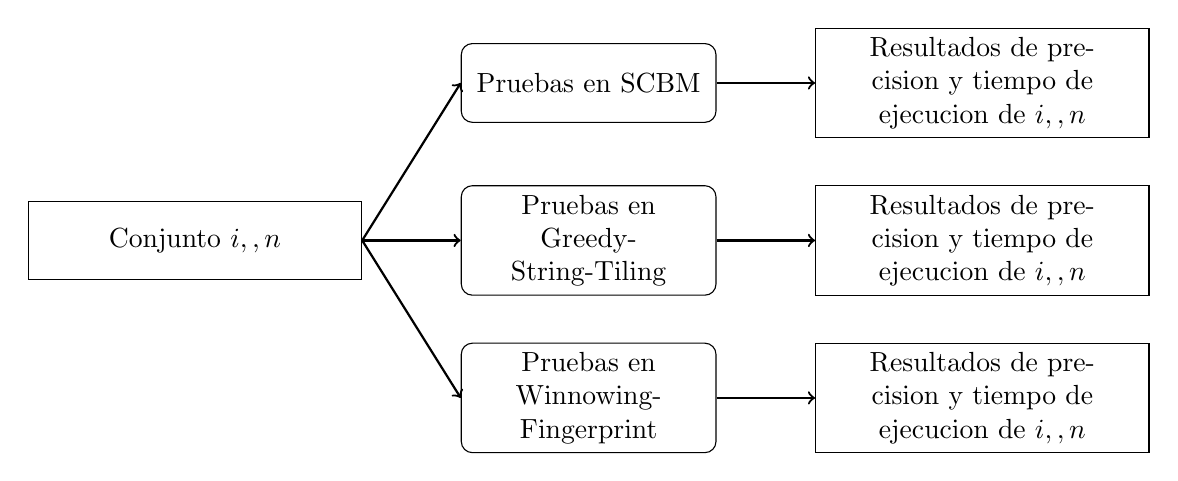
\begin{tikzpicture}[scale=1,
input_output/.style ={rectangle, minimum width=1cm, minimum height=1cm,text centered, text width=4cm, draw=black},
algorithm/.style={rectangle, rounded corners, minimum width=3cm, minimum height=1cm,text centered, text width=3cm, draw=black},
arrow/.style={thick,->,},
]
\node[input_output] (n0) at (1,3) {Conjunto $i, \twodots, n$};
\node[algorithm] (n1) at (6,1) {Pruebas en Winnowing-Fingerprint};
\node[algorithm] (n2) at (6,3) {Pruebas en Greedy-String-Tiling};
\node[algorithm] (n3) at (6,5) {Pruebas en SCBM};
\node[input_output] (n4) at (11,1) {Resultados de precision y tiempo de ejecucion de $i, \twodots, n$};
\node[input_output] (n5) at (11,3) {Resultados de precision y tiempo de ejecucion de $i, \twodots, n$};
\node[input_output] (n6) at (11,5) {Resultados de precision y tiempo de ejecucion de $i, \twodots, n$};
\draw [arrow] (n0.east) to (n1.west);
\draw [arrow] (n0.east) to (n2.west);
\draw [arrow] (n0.east) to (n3.west);
\draw [arrow] (n1.east) to (n4);
\draw [arrow] (n2.east) to (n5);
\draw [arrow] (n3.east) to (n6);
\end{tikzpicture}
\caption{Especificacion de las pruebas}
Fuente: Elaboración propia.
\label{espePrueba}
\end{figure}
